% !TEX root = ../main.tex

\section{Introduction}
\label{sec:introduction}
In this lab we will find out what striding and warps is all about. We learn how striding is useful in the code execution, why it should be implemented and what the benefits are. The next part of the lab is about warps where we will try to determine the impact of the thread size and limitations of CUDA.

The code repository can be found at: \\
\url{https://github.com/imstevenxyz/geavanceerde-computerarch}

\section{Striding}
\label{sec:striding}

To see the benefits of striding an image is generated using the given formula. This formula is implemented in two kernel functions, one that executes with striding and one without. Both are run with an amount of threads, the total pixels, a quarter of the total pixels and with more than the total pixels.

\begin{figure}[H]
    \centering
    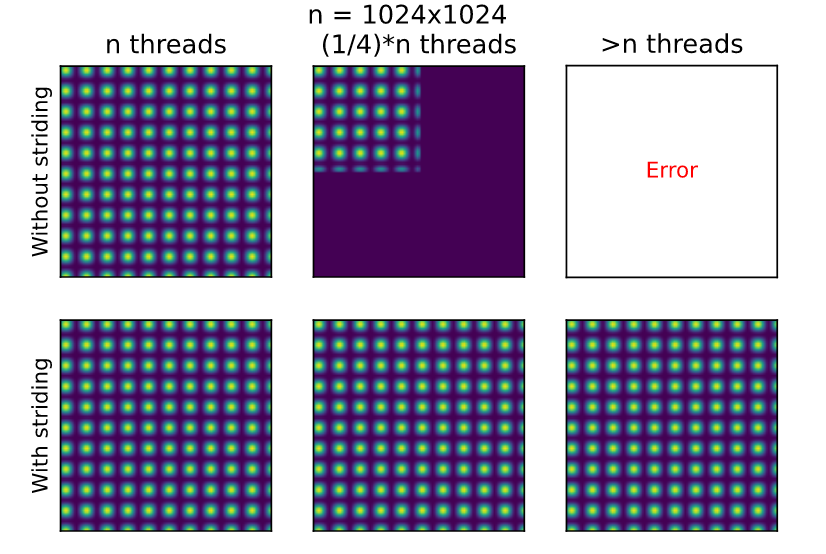
\includegraphics[width=0.5\textwidth]{images/striding.png}
    \caption{Timing performance semi parallel kernel}
    \label{figure:striding}
\end{figure}

It is directly obvious in figure \ref{figure:striding} that without striding we get three different results while with striding we get the wanted result for all variations. The outstanding in the figure is when we use more threads than pixel. In this variation the code will return an error because otherwise memory that does not belong to the image is accessed, this is either impossible or very dangerous (unwanted memory access, data theft, etc). When using a quarter of the pixels, only a quarter of the image is generated because the other pixels will not be calculated since there are not enough threads.

From this we can see that striding actually helps organize the threads in two ways:
\begin{itemize}
    \item Not enough threads? → Run threads sequentially.
    \item More than needed threads? → Do not run the calculations for non-existing memory locations.
\end{itemize}

\section{Warps}
\label{sec:warps}

A warp is a set of threads that work at the same time and execute the same code. The threads all share resources and they start and stop at the same time. This allows for better perfmance when the code is executed in warps. The size of a warp is depended on the architecture of the gpu and on the gpu we work on the warp size is 32 threads.

In the \ref{figure:warp_zoom} the execution time is plotted in function of the amount of threads used. This to show the effect of warp.
The Y-axis is the execution time.
The X-axis is the amount of threads used.
The names in the legends mean: 
B amount of blocks allocated (singular*)
T amount of threads allocated per block (singular)
I amount of pixels in the image (cubic)
(*the amount of blocks is actualy cubic in the code but we display it singular on the plot. This is to keep the numbers lower on the plot so its easier to see them, while reducing the computation time to get all the results. If interested in the real numbers you can open "plot_actual_threads.html" on the git.)

\begin{figure}[H]
    \centering
    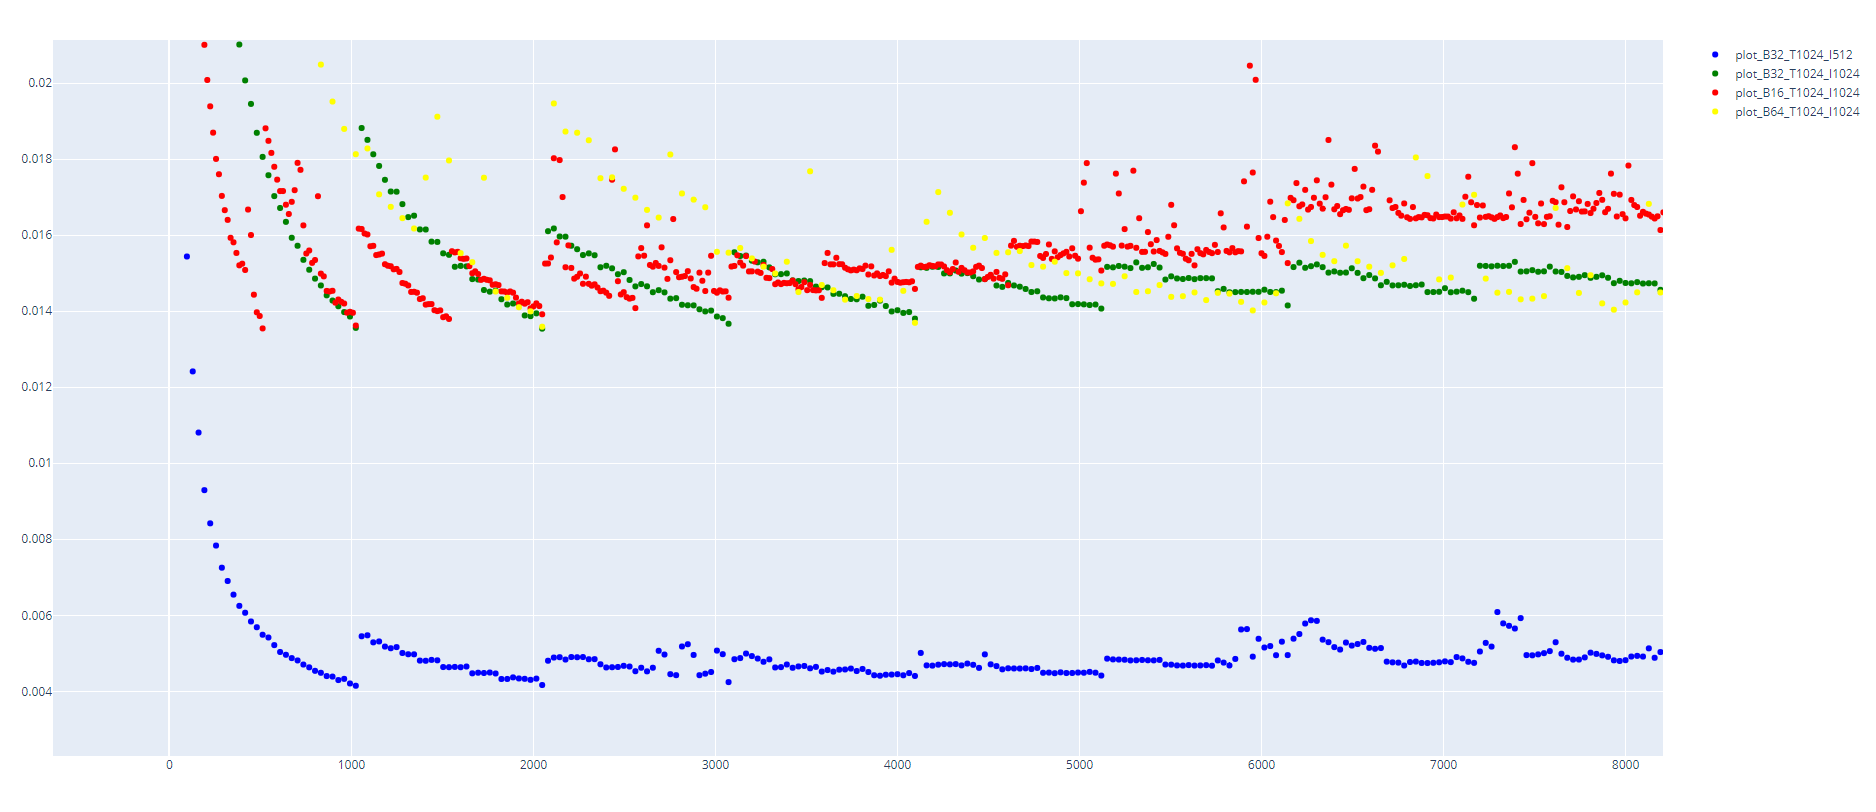
\includegraphics[width=0.5\textwidth]{images/warp_plot_zoom.PNG}
    \caption{Execution time in function of amount of threads}
    \label{figure:warp_zoom}
\end{figure}

In the \ref{figure:warp_zoom} we can see several intersting features pop up. Lets start with the 'waves'.You can see for all cases that there form something like 'waves'. The time drops the more threads are allocated and then suddendly jump up, and this patern repeats itself on regular interval. 
The repetition of the wave is because of the amount of blocks and the warp size. For B_16 it repeats every 512 threads, 16*32=512. For B_32 it repeats every 1024 threads, 32*32=1024. For B_64 it repeats every 2048 threads, 64*32=2048. 
The overal time increases because of the overhead of the large amount of threads that are used.
The blue plot B_32_T1024_I512 is faster just because the image is smaller so less needs to be calculated. The warp is still there and the patern is on the same interval as the green plot, the green plot has the same amount of blocks.

The waves (drop, jump, repeat) are there because 
The drop is there because in the interval the warps are not full so more threads do not require more resources, warp  will execute anyway. So any more threads can only reduce the amount of time that is required.
The jump is because once all the warps are full another set of warp needs to run. Another warp will require a lot more time even though there are more threads.
The repetition is there because the last warp, the unfilled one, is the bottleneck. And this only stops when you run out of threads.

\section{Conclusion}
\label{sec:conclusion}

With striding the code doesnt need to know beforehand how much blocks and threads needs to be allocated. The striding will work out if threads have to run the code multiple times or if threads dont have to run at all. And it will have somewhat of an even devision of the workload.
The warp has a impact on the time. More threads doesnt mean faster work. The threads should fill an entire warp, if not it will be slower and cost more resources.
